\section{Problemática}
\label{sec:problematica}

En los sistemas económicos contemporáneos, la declaración de ingresos por parte de las unidades empresariales constituye el insumo primordial tanto para la recaudación impositiva como para el cálculo del valor agregado bruto en el Sistema de Cuentas Nacionales. Sin embargo, en el contexto boliviano, las autoridades estatales enfrentan un dilema estructural derivado de la ausencia de herramientas computacionales avanzadas capaces de contrastar los valores monetarios declarados con la capacidad física real de producción observada en cada empresa informante.

Esta situación genera una asimetría de información que afecta a dos ámbitos estratégicos del Estado:
\begin{enumerate}
    \item \textbf{Consistencia Estadística de Cuentas Nacionales (INE):} Si las empresas medianas o grandes subdeclaran sus ingresos brutos para atenuar cargas fiscales o por deficiencias contables, las estimaciones agregadas del Producto Interno Bruto (PIB) sectorial subestiman la verdadera escala de la actividad económica boliviana, distorsionando las decisiones de política macroeconómica e inversión pública.
    \item \textbf{Equidad y Recaudación Tributaria (SIN):} La falta de un valor técnico esperado impide que las administraciones tributarias prioricen sus recursos de auditoría hacia aquellos contribuyentes que presentan discrepancias estadísticamente anómalas respecto a su dotación de capital, energía y fuerza de trabajo. Esto sobrecarga al personal fiscalizador en revisiones aleatorias de bajo rendimiento y vulnera el principio de equidad contributiva.
\end{enumerate}

Asimismo, desde el punto de vista del procesamiento de datos, los microdatos oficiales de la encuesta EAIMCS presentan desafíos cuantitativos considerables:
\begin{itemize}
    \item \textbf{Severa Asimetría y Colas Pesadas:} La distribución de los ingresos y de los activos fijos exhibe una marcada asimetría positiva (distribución de tipo Pareto), donde menos del 5\% de las empresas concentra más del 60\% de los ingresos agregados. Los modelos lineales convencionales colapsan ante esta dispersión extrema.
    \item \textbf{Presencia de Centinelas e Inconsistencias Contables:} Los datos brutos contienen códigos centinela (como el valor \texttt{99999.0}), utilizados por el INE para codificar registros con imputación pendiente o inconsistencia contable no resuelta, los cuales deben ser tratados sistemáticamente para no viciar el entrenamiento algorítmico.
    \item \textbf{Riesgo de Fuga de Información (\textit{Data Leakage}):} Existen variables calculadas por el INE con posterioridad a la encuesta (como el Valor Bruto de Producción o el Valor Agregado) y componentes contables directos que, de no ser excluidos explícitamente, contaminarían el modelo otorgándole un desempeño engañosamente perfecto pero inútil en un escenario de contraste ciego.
\end{itemize}

\subsection{a. Árbol de Problemas}
\label{subsec:arbol_problemas}

Para analizar sistemáticamente la cadena de causalidad que origina esta situación, se elaboró el \textbf{Árbol de Problemas} presentado en la Figura \ref{fig:arbol_problemas}. En este diagrama se desglosan los efectos de impacto que genera la falta de contraste objetivo, el problema central diagnosticado y las causas estructurales directas e indirectas que lo determinan.

\begin{figure}[htbp]
\centering
\caption{Árbol de Problemas: Diagnóstico de Causas y Efectos del Proyecto.}
\label{fig:arbol_problemas}
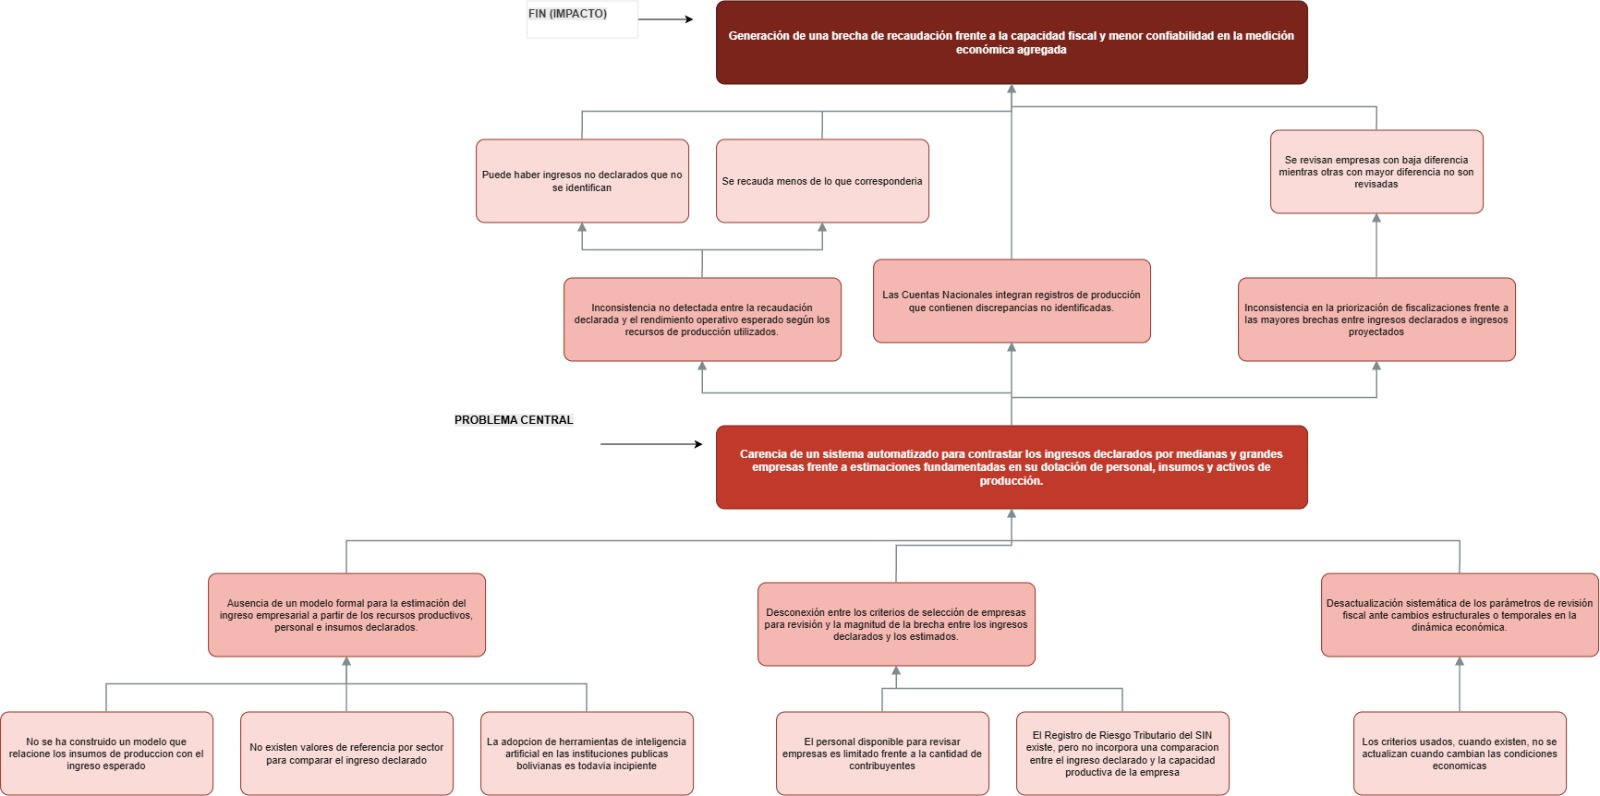
\includegraphics[width=\textwidth,keepaspectratio]{imagenes/arbol_problemas.jpg}
\vspace{1mm}
\raggedright\footnotesize
\textit{Nota.} Diagrama causal estructurado que identifica el problema central, causas directas e indirectas, y efectos de impacto en la consistencia fiscal y de Cuentas Nacionales.
\end{figure}

El diagnóstico sintetizado en la Figura \ref{fig:arbol_problemas} sitúa como \textbf{Problema Central} la \textit{carencia de un sistema automatizado para contrastar los ingresos declarados por medianas y grandes empresas frente a estimaciones fundamentadas en su dotación de personal, insumos y activos de producción}. Dicho problema se sustenta en tres causas estructurales directas:
\begin{enumerate}
    \item \textbf{Falta de un modelo formal multivariado:} No se ha construido previamente un modelo cuantitativo que relacione los insumos con el ingreso esperado, careciendo de valores de referencia sectoriales en un contexto donde la adopción de inteligencia artificial en instituciones públicas bolivianas es todavía incipiente.
    \item \textbf{Desconexión en los criterios de fiscalización:} El personal técnico disponible es limitado frente al universo de contribuyentes y el Registro de Riesgo Tributario del SIN no incorpora un contraste formal frente a la capacidad productiva de las empresas.
    \item \textbf{Desactualización sistemática de parámetros:} Los criterios de control fiscal, cuando existen, no se actualizan de manera continua y rigurosa ante fluctuaciones de la coyuntura económica y cambios estructurales.
\end{enumerate}

Esta configuración genera como impacto final una \textit{brecha de recaudación frente a la capacidad fiscal y menor confiabilidad en la medición económica agregada}, al permitir que existan ingresos no declarados no identificados, discrepancias no detectadas en los registros de Cuentas Nacionales y distorsiones en la priorización de auditorías tributarias.
